\chapter{METODE PENELITIAN}

\section{Gambaran Umum Penelitian}

Penelitian ini bertujuan untuk mengembangkan dan mengevaluasi sebuah \textit{framework} adaptif untuk pemetaan terminologi klinis Bahasa Indonesia ke kosakata terkendali standar, seperti SNOMED CT, LOINC, dan ICD-10. Pendekatan utama yang diusulkan adalah adaptasi dari arsitektur CDE-Mapper \citep{gilani_cde-mapper_2025} dengan optimalisasi komponen ekstraksi teks klinis yang menggunakan bahasa Indonesia dan berupa teks panjang.

\section{Tahapan Penelitian}

Penelitian ini akan dilaksanakan dalam lima tahapan utama seperti digambarkan pada Gambar~\ref{fig:tahapan-penelitian}.


\begin{figure}[H]
    \centering
    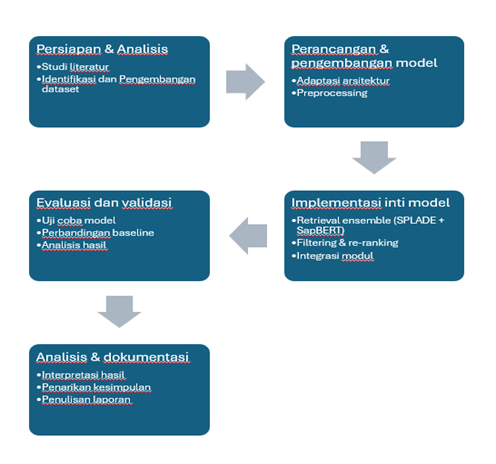
\includegraphics[width=0.8\textwidth]{media/tahapan_penelitian.png}
    \caption{Tahapan penelitian}
    \label{fig:tahapan-penelitian}
\end{figure}

Penelitian ini dilaksanakan dalam lima tahapan utama yang saling terkait secara berurutan maupun iteratif. Kelima tahapan pada Gambar~\ref{fig:tahapan-penelitian} dijelaskan sebagai berikut.

\subsection{Persiapan dan Analisis}

Tahap ini bertujuan untuk membangun fondasi teoritis dan menyiapkan sumber daya data yang diperlukan sebelum memasuki pengembangan model.

\subsubsection{Studi Literatur}

Studi literatur dilakukan secara sistematis untuk mengidentifikasi \textit{state-of-the-art} dalam pemetaan terminologi klinis. Ruang lingkup literatur mencakup standar interoperabilitas kesehatan, seperti FHIR, SNOMED CT, LOINC, dan ICD-10, serta implementasinya di SATUSEHAT \citep{ayuningtyas_bringing_2025,heryawan_fast_2025}; metode pemetaan dari \textit{rule-based}, \textit{machine learning}, \textit{deep learning}, hingga LLM dan RAG \citep{meizoso_automated_2011,hristov_application_2021,gilani_cde-mapper_2025}; serta arsitektur CDE-Mapper dan keterbatasannya dalam memproses teks panjang dengan \textit{multiple CDE} komposit \citep{gilani_cde-mapper_2025}. Hasil studi literatur digunakan untuk merumuskan kerangka konseptual dan menentukan komponen kunci yang akan diadaptasi.

\subsubsection{Identifikasi dan Pengembangan Dataset}

Kegiatan ini mencakup identifikasi sumber data istilah klinis Bahasa Indonesia. Data diperoleh dari rekam medis elektronik (RME) puskesmas atau klinik swasta, dan platform konsultasi kesehatan daring yang telah dianonimkan. Sumber-sumber ini dipilih karena merepresentasikan variasi nyata istilah lokal, singkatan, dan kesalahan eja \citep{purwitasari_comparison_2023,hossain_exploratory_2025}. Selain itu, dikumpulkan pula kosakata terkendali standar berupa SNOMED CT, LOINC, dan ICD-10 sebagai terminologi target.

Pembangunan dataset emas (\textit{gold standard}) dilakukan dengan menganotasi sampel 100--200 istilah klinis secara manual oleh tenaga medis, seperti dokter atau perekam medis, dengan kode standar yang sesuai. Validasi antar-anotator (\textit{inter-annotator agreement}) dihitung menggunakan koefisien Kappa Fleiss untuk menjamin konsistensi. Dataset emas ini menjadi kebenaran dasar untuk evaluasi performa model.

\subsection{Perancangan dan Pengembangan Model}

Pada tahap ini, arsitektur model usulan dirancang dan komponen \textit{preprocessing} dikembangkan secara spesifik untuk teks klinis panjang dalam bahasa Indonesia.

\subsubsection{Adaptasi Arsitektur}

Arsitektur CDE-Mapper diadaptasi dengan penambahan modul dekomposisi teks panjang dalam bahasa Indonesia. Karena CDE-Mapper asli hanya menerima satu CDE per \textit{input}, ditambahkan modul yang memecah dokumen klinis panjang menjadi unit-unit kalimat atau klausa yang mengandung CDE potensial. Pendekatan ini menggunakan aturan pemisah kalimat, dan deteksi frasa klinis berbasis pola.

Optimasi \textit{LLM-based query decomposition} untuk \textit{retrieval ensemble} dilakukan agar sesuai dengan karakteristik istilah klinis Bahasa Indonesia dan kebutuhan \textit{multi-terminology mapping}. Selain itu, diintegrasikan pula mekanisme \textit{confidence-based selection} yang diadaptasi dari pendekatan hibrida normalisasi konsep klinis oleh \citet{chen_clinical_2020} untuk menangani ketidakpastian dan merekomendasikan kandidat yang perlu validasi manual.

\subsubsection{Preprocessing}

\textit{Preprocessing} dirancang khusus untuk membersihkan dan menstandarkan teks klinis sebelum masuk ke pemrosesan lanjutan. Langkah-langkahnya meliputi \textit{case folding} (semua teks diubah menjadi huruf kecil); normalisasi singkatan medis menggunakan kamus singkatan yang dibangun dari literatur dan buku rekam medis, misalnya DM'' menjadidiabetes mellitus'' dan TD'' menjaditekanan darah''; \textit{stemming} Bahasa Indonesia untuk mengurangi kata berimbuhan ke bentuk dasar secara selektif; penanganan variasi ejaan dan istilah sehari-hari; serta segmentasi kalimat untuk menjaga konteks lokal setiap entitas. Tahap ini hanya bertujuan menyiapkan teks bersih dan tidak melakukan pemetaan konsep.

\subsection{Implementasi Inti Model}

Implementasi inti model dibangun dalam sebuah \textit{pipeline} berbasis Python yang mengintegrasikan enam komponen utama secara berurutan. Pertama, ekstraksi multi-entitas dari teks klinis menjadi objek JSON terstruktur, yang memuat entitas utama, domain, kategori, unit, metode, negasi, dan konteks temporal. Kedua, penerapan aturan pemetaan berbasis domain untuk menentukan terminologi target (SNOMED CT, LOINC, atau ICD-10), dilanjutkan dengan dekomposisi kueri menjadi komponen atomik guna menghindari ambiguitas pencarian. Ketiga, pemeriksaan \textit{knowledge reservoir} untuk mengambil hasil tervalidasi jika tersedia dan menghindari komputasi ulang. Keempat, \textit{retrieval ensemble} yang memanfaatkan SPLADE untuk pencarian leksikal dan SapBERT untuk pencarian semantik, guna menghasilkan daftar kandidat konsep standar dari basis pengetahuan terminologi. Kelima, \textit{filtering} dan \textit{re-ranking} untuk menyaring kandidat yang tidak sesuai domain, atribut, atau status aktif, serta menilai ulang kesesuaiannya terhadap konteks kalimat secara keseluruhan. Keenam, validasi keputusan melalui agregasi penilaian, dengan keluaran akhir berupa kandidat final beserta skor kepercayaan, atau status \textit{abstain} yang memerlukan validasi ahli jika tidak ada kandidat yang memenuhi ambang penerimaan.

\subsection{Evaluasi dan Validasi}

Tahap ini menguji performa model secara kuantitatif dan kualitatif.

\subsubsection{Uji Coba Model}

Model diuji pada dataset emas dengan skenario sebagai berikut.

\begin{enumerate}
    \item Uji standar: menggunakan istilah yang sudah baku dalam dataset.
    \item Uji variasi leksikal: menggunakan istilah dengan singkatan, ejaan salah, atau bahasa sehari-hari yang diambil dari platform konsultasi daring \citep{purwitasari_comparison_2023}.
    \item Uji teks panjang: menggunakan dokumen klinis naratif, misalnya catatan perkembangan pasien, yang mengandung beberapa CDE komposit. Model harus mengekstraksi seluruh CDE dan memetakannya.
    \item Uji ablasi: model dijalankan tanpa komponen tertentu, yaitu tanpa modul \textit{rule-based}, tanpa SapBERT, dan tanpa \textit{cross-encoder}, untuk mengukur kontribusi masing-masing komponen.
    \item Perbandingan \textit{baseline}: perbandingan utama yang akan dilakukan adalah membandingkan \textit{framework} usulan dengan CDE-Mapper original \citep{gilani_cde-mapper_2025}. Jika memungkinkan, simulasi dengan LLM kecil akan digunakan untuk proses dekomposisi dengan anggaran komputasi yang dibatasi.
\end{enumerate}

\subsubsection{Analisis Hasil}

Hasil kuantitatif disajikan dalam tabel dan grafik perbandingan. Analisis statistik, misalnya uji-\textit{t} berpasangan, dilakukan untuk menentukan signifikansi perbedaan antar model. Selain itu, dilakukan analisis kesalahan (\textit{error analysis}) dengan mengelompokkan kesalahan pemetaan ke dalam kategori berikut.

\begin{enumerate}
    \item Kesalahan karena variasi leksikal, misalnya singkatan yang tidak dikenal.
    \item Kesalahan karena ambiguitas semantik, yaitu satu istilah dapat merujuk ke dua konsep berbeda.
    \item Kesalahan karena kegagalan ekstraksi CDE dari teks panjang.
    \item Kesalahan karena keterbatasan pengetahuan terminologi, yaitu ketika konsep tidak ada di basis data.
\end{enumerate}

Setiap kesalahan dianalisis secara kualitatif untuk memberikan rekomendasi perbaikan.

\subsection{Analisis dan Dokumentasi}

Tahap akhir penelitian ini berfokus pada interpretasi, penarikan kesimpulan, dan penulisan laporan.

\subsubsection{Interpretasi Hasil}

Hasil evaluasi diinterpretasikan dalam kerangka pertanyaan penelitian: seberapa baik \textit{framework} usulan memetakan terminologi klinis Bahasa Indonesia dibandingkan \textit{baseline}; bagaimana kontribusi masing-masing komponen, seperti dekomposisi, \textit{retrieval ensemble}, dan \textit{preprocessing}, terhadap peningkatan akurasi; apakah model mampu menangani teks panjang dengan \textit{multiple CDE} komposit secara simultan; dan seberapa efisien model digunakan untuk teks klinis dalam bahasa Indonesia.

\subsubsection{Penarikan Kesimpulan}

Kesimpulan dirumuskan berdasarkan tujuan penelitian yang ditetapkan di Bab I. \textit{Framework} adaptif yang dikembangkan diharapkan mampu mengatasi keterbatasan CDE-Mapper asli dalam memproses teks klinis panjang dan mengenali \textit{multiple CDE}. Pendekatan \textit{hybrid rule-based} dan \textit{semantic retrieval} diharapkan efektif untuk konteks \textit{low-resource} bahasa Indonesia dengan akurasi yang kompetitif. Rekomendasi juga diberikan untuk implementasi di SATUSEHAT dan penelitian lanjutan, termasuk perlunya validasi klinis yang lebih luas dan pengembangan mekanisme \textit{active learning} untuk memperbaiki model secara berkelanjutan.

\subsubsection{Penulisan Laporan}

Seluruh proses, desain, implementasi, data, hasil, dan kesimpulan didokumentasikan secara sistematis dalam naskah disertasi sesuai panduan penulisan Universitas Gadjah Mada. Laporan juga mencakup kode sumber pada repositori pendukung dan dataset anonim yang digunakan sehingga penelitian ini dapat direproduksi dan dikembangkan lebih lanjut oleh peneliti lain.

\section{Deskripsi Usulan Model}

Arsitektur model yang diusulkan untuk mengadaptasi CDE-Mapper agar mampu melakukan pemetaan terminologi klinis secara \textit{end-to-end} dari teks klinis panjang berbahasa Indonesia, menjadi kode standar, yaitu SNOMED CT, LOINC, dan ICD-10. Model diusulkan sebagai \textit{pipeline hybrid} yang menggabungkan ekstraksi entitas berbasis LLM, \textit{retrieval} semantik dan leksikal (\textit{dense} + \textit{sparse}), serta mekanisme validasi dan penyimpanan pengetahuan (\textit{knowledge reservoir}) untuk meningkatkan akurasi dan efisiensi inferensi \citep{gilani_cde-mapper_2025}.

\subsection{Tujuan dan Keluaran Model}

Secara operasional, model menerima masukan berupa: (1) teks klinis panjang berbahasa Indonesia, misalnya resume medis, catatan perkembangan, atau hasil penunjang; atau (2) daftar istilah atau \textit{field} dari kamus data RME. Keluaran yang diharapkan adalah daftar \textit{clinical data elements} (CDE) hasil ekstraksi beserta pasangan pemetaan ke terminologi target, yang mencakup \textit{mention} asli, tipe entitas, normalisasi istilah, kandidat kode teratas (Top-\textit{k}), skor kepercayaan, serta keputusan akhir, yaitu \textit{exact}, \textit{highly}, \textit{partial}, atau \textit{not relevant}. Untuk kasus komposit, keluaran juga menyertakan dekomposisi atribut, yaitu \textit{Base entity}, \textit{Domain}, \textit{Additional Entities}, \textit{categories}, \textit{Unit}, \textit{Visit}, dan \textit{Method} \citep{gilani_cde-mapper_2025}.


\subsection{Arsitektur, Alur Proses, dan Komponen Utama}

Arsitektur usulan mengadopsi komponen utama CDE-Mapper \citep{gilani_cde-mapper_2025}, kemudian menambahkan lapisan NLP untuk mengubah teks klinis naratif berbahasa Indonesia menjadi sekumpulan CDE terstruktur. Adaptasi ini berfokus pada: (i) penanganan variasi bahasa klinis Indonesia, seperti singkatan, istilah lokal, ejaan tidak baku, negasi, dan konteks temporal; (ii) pemrosesan teks panjang yang dapat mengandung banyak entitas, bukan hanya satu CDE pada setiap masukan; dan (iii) pemetaan ke tiga terminologi dalam ruang lingkup penelitian, yaitu SNOMED CT, LOINC, dan ICD-10.

Secara operasional, arsitektur merupakan rangkaian delapan langkah: pra-pemrosesan dan normalisasi bahasa; ekstraksi multi-entitas dan pembentukan JSON; penerapan \textit{mapping rules} serta transformasi format; dekomposisi kueri secara \textit{batch}; pemeriksaan \textit{knowledge reservoir}; \textit{ensemble retrieval}; \textit{filtering}, \textit{reranking}, dan validasi; serta pembaruan \textit{knowledge reservoir}. Rangkaian tersebut menghubungkan modul NLP yang menjadi kontribusi adaptasi dengan algoritma CDE-Mapper.

\begin{figure}[H]
    \centering
    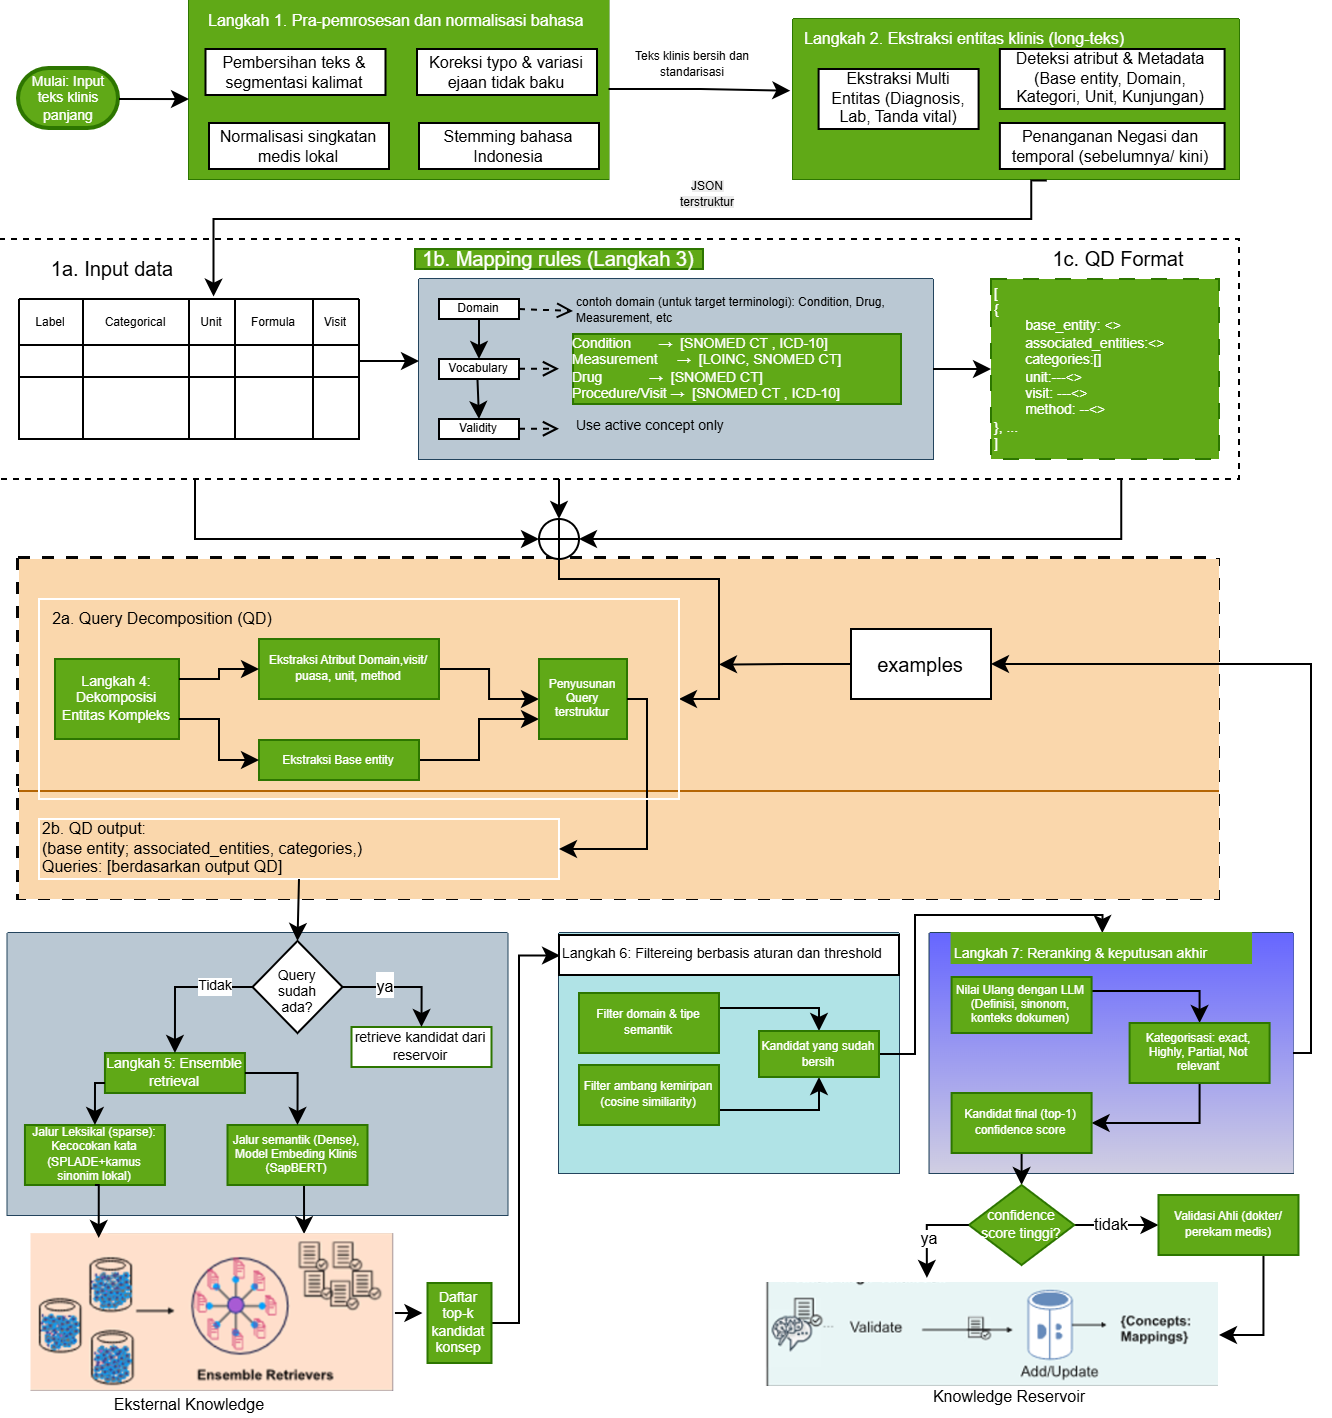
\includegraphics[width=0.95\textwidth]{media/Framework Usulan 25062026-Rev2 Agst.png}
    \caption{Framework adaptasi pemetaan terminologi klinis Bahasa Indonesia}
    \label{fig:alur-operasional-mapping}
\end{figure}

Bagian berarsir hijau pada Gambar~\ref{fig:alur-operasional-mapping} menunjukkan komponen yang ditambahkan atau disesuaikan untuk Bahasa Indonesia. Penjelasan setiap langkah adalah sebagai berikut.

\Needspace{6\baselineskip}
\begin{enumerate}
    \item \textbf{Pra-pemrosesan dan normalisasi bahasa.}
    \begin{itemize}
        \item \textbf{Fungsi:} membersihkan teks, melakukan segmentasi kalimat, memperbaiki ejaan tidak baku, menormalkan singkatan medis, melakukan \textit{stemming}, serta menstandarkan simbol, angka, dan satuan tanpa menghilangkan informasi klinis penting.
        \item \textbf{Pembersihan teks:} karakter berulang, emotikon, spasi berlebih, dan pemisah baris yang tidak informatif dibersihkan. Implementasi awal dapat memanfaatkan dan menyesuaikan modul \textit{text-normalization} untuk karakteristik data klinis \citep{utomo_text_normalization}.
        \item \textbf{Segmentasi kalimat:} dokumen panjang dibagi menjadi kalimat atau segmen koheren agar konteks lokal setiap entitas tetap terjaga. Model segmentasi berbasis transformer untuk Bahasa Indonesia dapat digunakan sebagai acuan atau pembanding \citep{Hananto2026}.
        \item \textbf{Koreksi bentuk tidak baku:} variasi informal, salah eja, dan pengulangan huruf dinormalkan menggunakan kamus dan aturan yang dapat diadaptasi dari \textit{indo-normalizer} \citep{dyasputro_indo_normalizer}.
        \item \textbf{Normalisasi singkatan medis:} singkatan seperti ``Px'', ``dgn'', ``DM'', ``GDP'', dan ``TD'' diperluas menggunakan kamus singkatan medis lokal. Kamus awal mengacu pada daftar singkatan rekam medis dan selanjutnya divalidasi oleh ahli \citep{RSI_Sultan_Agung_2019}.
        \item \textbf{Stemming selektif:} kata berimbuhan dapat dikembalikan ke bentuk dasar menggunakan Sastrawi \citep{librian_sastrawi}. Stemming tidak diterapkan pada kode, nama obat, nilai numerik, dan istilah yang berisiko berubah makna klinis.
        \item \textbf{Contoh input:} ``Px dgn DM tipe 2, GDP 126 mg/dL, TD 150/90''.
        \item \textbf{Contoh keluaran:} ``pasien dengan diabetes mellitus tipe 2, gula darah puasa 126 mg/dL, tekanan darah 150/90''.
        \item \textbf{Keluaran tahap:} teks klinis bersih yang siap diproses oleh modul ekstraksi entitas.
    \end{itemize}

    \Needspace{6\baselineskip}
    \item \textbf{Ekstraksi multi-entitas dan pembentukan JSON.}
    \begin{itemize}
        \item \textbf{Fungsi:} mendeteksi banyak entitas klinis dari setiap segmen menggunakan LLM atau model NER medis. Model medis yang menyediakan keluaran NER terstruktur, seperti Numind Medical NER LLM, dapat digunakan sebagai salah satu kandidat dan dibandingkan dengan LLM melalui pendekatan \textit{few-shot} \citep{johnsnowlabs2026numind}.
        \item \textbf{Informasi yang dideteksi:} entitas utama, domain, kategori atau nilai kategorikal, unit, metode atau formula, kunjungan, atribut tambahan, status negasi, dan konteks temporal. Instruksi atau aturan khusus digunakan agar frasa seperti ``tidak ada'', ``bukan'', dan ``tanpa'' ditandai sebagai negasi, sedangkan ``sebelumnya'', ``dulu'', ``kini'', dan ``saat ini'' diberi penanda waktu.
        \item \textbf{Output terstruktur:} setiap entitas disimpan sebagai objek JSON. \textit{Label} memuat nama CDE atau frasa klinis utama; \textit{categorical} memuat daftar atau pasangan kategori nilai; \textit{unit} memuat satuan pengukuran; \textit{formula} memuat aturan perhitungan atau hubungan antarelemen apabila CDE merupakan hasil turunan; dan \textit{visit} memuat konteks kunjungan atau waktu pengukuran. Metadata tambahan seperti \textit{domain}, \textit{method}, \textit{assertion}, dan \textit{temporal} dipertahankan untuk membantu pemetaan.
        \item \textbf{Contoh hasil:} ``diabetes mellitus tipe 2'' sebagai diagnosis; ``gula darah puasa 126 mg/dL'' sebagai pemeriksaan laboratorium; dan ``tekanan darah 150/90'' sebagai tanda vital.
        \item \textbf{Keluaran tahap:} daftar \textit{mention} terstruktur sehingga satu dokumen panjang dapat menghasilkan beberapa CDE sekaligus \citep{purwitasari_comparison_2023}.
    \end{itemize}

    \Needspace{6\baselineskip}
    \item \textbf{Penerapan \textit{mapping rules} dan transformasi format.}
    \begin{itemize}
        \item \textbf{Fungsi:} memeriksa domain entitas, menentukan terminologi target, membatasi pencarian pada konsep aktif, dan mengubah setiap objek JSON ke format masukan dekomposisi kueri.
        \item \textbf{Aturan terminologi:} domain \textit{condition}, temuan klinis, prosedur, dan kunjungan diprioritaskan ke SNOMED CT; domain \textit{measurement} diprioritaskan ke LOINC dengan SNOMED CT sebagai alternatif jika sesuai; dan diagnosis untuk kebutuhan klasifikasi atau pelaporan diarahkan ke ICD-10. Entitas obat berada di luar terminologi obat khusus pada ruang lingkup penelitian ini; pemetaan hanya dilakukan apabila tersedia konsep aktif yang sesuai dalam SNOMED CT, sedangkan kasus lainnya ditandai untuk perluasan penelitian.
        \item \textbf{Validitas kandidat:} hanya konsep yang berstatus aktif dalam versi terminologi yang digunakan yang dimasukkan ke ruang pencarian, mengikuti prinsip penyaringan pada CDE-Mapper \citep{gilani_cde-mapper_2025}.
        \item \textbf{Contoh:} ``diabetes mellitus tipe 2'' diarahkan ke SNOMED CT dan ICD-10, sedangkan ``gula darah puasa'' diarahkan ke LOINC.
        \item \textbf{Keluaran tahap:} beberapa set JSON, masing-masing mewakili satu entitas beserta metadata dan terminologi targetnya. Format tersebut mengikuti kebutuhan \textit{linking rules} yang dapat dikonfigurasi untuk konteks SATUSEHAT \citep{ayuningtyas_bringing_2025}.
    \end{itemize}

    \Needspace{0.45\textheight}
    \item \textbf{Dekomposisi kueri secara \textit{batch}.}
    \begin{itemize}
        \item \textbf{Fungsi:} memecah setiap entitas kompleks menjadi komponen logis dan unit pencarian atomik agar kueri tidak ambigu atau terlalu spesifik \citep{gilani_cde-mapper_2025}.
        \item \textbf{Contoh entitas:} ``gula darah puasa 126 mg/dL''.
        \item \textbf{Contoh dekomposisi:} \textit{base entity} = glukosa; \textit{domain} = pengukuran laboratorium; \textit{context} = puasa; dan \textit{unit} = mg/dL.
        \item \textbf{Adaptasi:} CDE-Mapper memproses satu baris kamus data pada setiap proses, sedangkan arsitektur usulan menjalankan dekomposisi untuk $N$ entitas yang diekstraksi dari satu dokumen. Karena itu, keluaran tahap ini berupa struktur JSON terdekomposisi dan daftar subkueri untuk seluruh entitas.
        \item \textbf{Keluaran tahap:} sekumpulan subkueri terstruktur yang mengarahkan pencarian pada konsep dan atribut yang tepat, bukan sekadar kecocokan satu kata.
    \end{itemize}

    \Needspace{6\baselineskip}
    \item \textbf{Pemeriksaan \textit{knowledge reservoir}.}
    \begin{itemize}
        \item \textbf{Fungsi:} memeriksa apakah kueri dan konteksnya telah memiliki pemetaan yang divalidasi ahli. Mekanisme ini diadopsi untuk mengurangi biaya komputasi dan latensi \citep{gilani_cde-mapper_2025}.
        \item \textbf{\textit{Cache hit}:} hasil tervalidasi diambil langsung tanpa menjalankan \textit{retrieval} dan \textit{reranking} ulang, setelah kesesuaian konteks, domain, dan versi terminologi diperiksa.
        \item \textbf{\textit{Cache miss}:} kueri diteruskan ke \textit{ensemble retrieval}, \textit{filtering}, \textit{reranking}, dan validasi.
        \item \textbf{Keluaran tahap:} hasil pemetaan tervalidasi atau subkueri yang perlu diproses oleh tahap pencarian.
    \end{itemize}

    \Needspace{6\baselineskip}
    \item \textbf{\textit{Ensemble retrieval} kandidat konsep.}
    \begin{itemize}
        \item \textbf{Fungsi:} mengambil kandidat dari basis pengetahuan terminologi melalui jalur leksikal dan semantik yang saling melengkapi.
        \item \textbf{\textit{Sparse retrieval}:} SPLADE membentuk representasi jarang pada ruang kosakata dan memberi bobot pada token penting serta ekspansi leksikal. Jalur ini efektif untuk istilah teknis, singkatan, dan kecocokan kata yang spesifik \citep{formal_splade_2021}. Skor kandidat mengikuti formulasi \textit{sparse retrieval} pada Persamaan~\ref{eq:sparse-retrieval}.
        \item \textbf{\textit{Dense retrieval}:} SapBERT membentuk representasi padat untuk menangkap sinonim dan kemiripan makna, misalnya hubungan antara ``gula darah puasa'' dan \textit{fasting blood glucose} \citep{liu_self-alignment_2021}. Kemiripan dihitung menggunakan Persamaan~\ref{eq:dense-retrieval}.
        \item \textbf{Penggabungan hasil:} kedua daftar kandidat digabungkan agar kandidat yang kuat secara leksikal maupun semantik memperoleh prioritas. Implementasi fusi dan bobotnya ditentukan pada data pengembangan sebagaimana Persamaan~\ref{eq:hybrid-retrieval}; metode tersebut merupakan pilihan implementasi penelitian dan tidak dinyatakan sebagai metode fusi asli Gilani.
        \item \textbf{Keluaran tahap:} daftar Top-\textit{k} kandidat aktif dari terminologi target yang telah diperkaya sinonim \citep{gilani_cde-mapper_2025}.
    \end{itemize}

    \Needspace{6\baselineskip}
    \item \textbf{\textit{Filtering}, \textit{reranking}, dan validasi keputusan.}
    \begin{itemize}
        \item \textbf{Filtering:} kandidat yang tidak sesuai domain, tipe semantik, status aktif, atribut, atau ambang kemiripan dieliminasi. Sebagai contoh, kandidat glukosa urin atau glukosa sewaktu dibuang ketika spesimen atau konteks puasa tidak sesuai. Ambang seperti \textit{cosine similarity} dapat membantu mengendalikan kandidat yang masuk ke tahap berikutnya \citep{chen_clinical_2020}.
        \item \textbf{Reranking:} kandidat tersisa dinilai ulang menggunakan LLM atau model \textit{reranker} dengan mempertimbangkan label, definisi, sinonim, domain, atribut, granularitas, negasi, konteks temporal, dan konteks kalimat.
        \item \textbf{Kategori keputusan:} \textit{exact}, \textit{highly}, \textit{partial}, atau \textit{not relevant}.
        \item \textbf{Contoh:} ``diabetes mellitus tipe 2'' diberi label \textit{exact} untuk SNOMED CT 44054006 dan ICD-10 E11.9, sedangkan ``diabetes mellitus'' tanpa tipe diberi label \textit{partial}.
        \item \textbf{Validasi keputusan:} penilaian dapat diulang dan diagregasi melalui \textit{self-consistency} untuk meningkatkan kestabilan \citep{wang_self-consistency_2023,gilani_cde-mapper_2025}. Kandidat yang tidak memenuhi ambang penerimaan menghasilkan keputusan \textit{abstain} dan diteruskan kepada ahli.
        \item \textbf{Keluaran tahap:} kandidat final Top-1 dan Top-\textit{k}, label relevansi, skor kepercayaan, serta status diterima atau memerlukan validasi ahli.
    \end{itemize}

    \Needspace{6\baselineskip}
    \item \textbf{Pembaruan \textit{knowledge reservoir} dan keluaran.}
    \begin{itemize}
        \item \textbf{Fungsi:} menyimpan pasangan \textit{mention}, konteks, metadata, terminologi target, dan kode standar yang telah divalidasi ahli.
        \item \textbf{Contoh simpanan:} ``DM tipe 2''--SNOMED CT 44054006 dan ``DM tipe 2''--ICD-10 E11.9.
        \item \textbf{Manfaat:} mempercepat pemetaan istilah berulang dan meningkatkan konsistensi lintas dokumen.
        \item \textbf{Peran \textit{human-in-the-loop}:} hasil dengan keyakinan rendah, konflik terminologi, atau keputusan \textit{abstain} divalidasi oleh dokter atau perekam medis sebelum disimpan. Dengan demikian, reservoir tidak otomatis menerima keluaran model yang belum diverifikasi.
        \item \textbf{Keluaran tahap:} daftar pemetaan terminologi untuk dokumen masukan dan referensi tervalidasi bagi inferensi berikutnya. Pemeriksaan konteks dan versi terminologi tetap dilakukan untuk mencegah penggunaan ulang pemetaan yang tidak sesuai \citep{gilani_cde-mapper_2025}.
    \end{itemize}
\end{enumerate}

Contoh alur \textit{end-to-end}: masukan \textit{``Px dgn DM tipe 2, GDP 126 mg/dL, TD 150/90''} akan dinormalisasi menjadi istilah baku, dipecah menjadi tiga entitas klinis, diarahkan ke terminologi target yang berbeda, kemudian menghasilkan kandidat seperti SNOMED CT 44054006 atau ICD-10 E11.9 untuk diagnosis diabetes mellitus tipe 2 serta kandidat LOINC untuk observasi glukosa puasa. Dengan demikian, satu dokumen klinis panjang dapat menghasilkan beberapa pemetaan standar secara simultan.

Arsitektur dan alur \textit{pipeline} yang diusulkan secara visual dapat dilihat pada Gambar~\ref{fig:arsitektur-usulan-model}.

\begin{figure}[H]
    \centering
    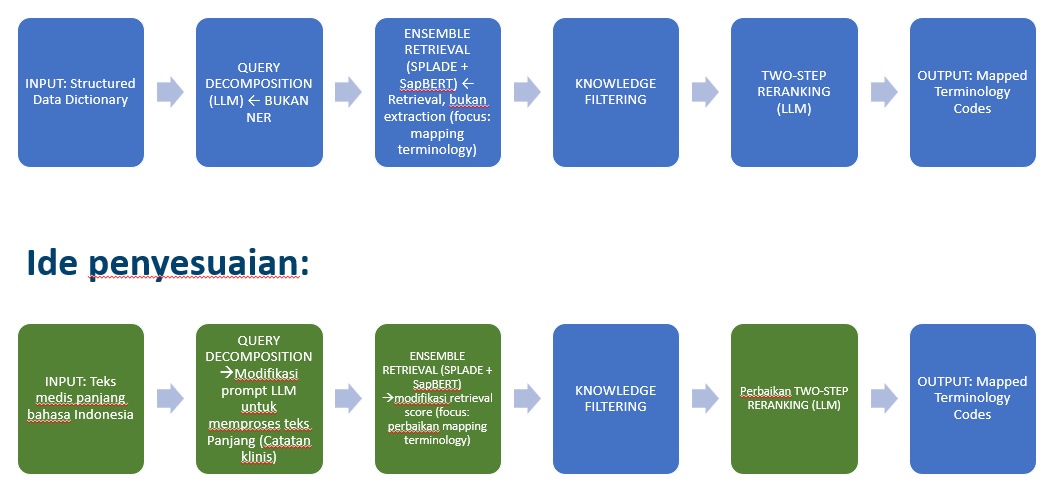
\includegraphics[width=0.9\textwidth]{prism-uploads/image.png}
    \caption{Gambaran arsitektur dan alur \textit{pipeline} yang diusulkan}
    \label{fig:arsitektur-usulan-model}
\end{figure}

\newcounter{algoritma}[chapter]
\renewcommand{\thealgoritma}{\arabic{chapter}.\arabic{algoritma}}

\textit{Pseudo code} pada Algoritma~\ref{alg:pemetaan-terminologi} merangkum alur operasional model dari masukan teks klinis sampai terbentuknya keluaran pemetaan dan pembaruan \textit{knowledge reservoir}.

\par
\begingroup
\scriptsize
\setstretch{1}
\renewcommand{\LTcaptype}{algoritma}
\providecommand{\theHalgoritma}{\theHchapter.\arabic{algoritma}}
\setlength{\tabcolsep}{0pt}
\newcommand{\algtext}[2]{\hspace*{#1em}\parbox[t]{\dimexpr\linewidth-#1em\relax}{\raggedright #2\strut}}
\Needspace{12\baselineskip}
\begin{longtable}{@{}p{1.8em}@{\hspace{0.6em}}p{\dimexpr0.96\textwidth-2.4em\relax}@{}}
\hline
\multicolumn{2}{@{}p{0.96\textwidth}@{}}{\textbf{Algoritma~\thealgoritma. Pemetaan Terminologi Klinis Bahasa Indonesia}\label{alg:pemetaan-terminologi}}\\
\hline
\multicolumn{2}{@{}p{0.96\textwidth}@{}}{\textbf{Masukan:} teks klinis panjang atau daftar istilah RME; basis pengetahuan SNOMED CT, LOINC, ICD-10; \textit{knowledge reservoir}; aturan pemetaan; dan parameter model.}\\
\multicolumn{2}{@{}p{0.96\textwidth}@{}}{\textbf{Keluaran:} hasil pemetaan dan antrean validasi ahli.}\\[0.5em]
\endfirsthead
\hline
\multicolumn{2}{@{}p{0.96\textwidth}@{}}{\textbf{Algoritma~\thealgoritma. Pemetaan Terminologi Klinis Bahasa Indonesia (lanjutan)}}\\
\hline
\endhead
\multicolumn{2}{@{}r@{}}{\textit{Bersambung ke halaman berikutnya.}}\\
\hline
\endfoot
\hline
\endlastfoot
1. & \algtext{0}{$teks\_bersih \leftarrow$ pra-pemrosesan dan normalisasi bahasa($teks\_masukan$)}\\*
2. & \algtext{0}{$daftar\_entitas \leftarrow$ ekstraksi multi-entitas dan metadata ke JSON($teks\_bersih$)}\\*
3. & \algtext{0}{$masukan\_QD \leftarrow$ penerapan \textit{mapping rules} dan transformasi format($daftar\_entitas$)}\\*
4. & \algtext{0}{$daftar\_tugas \leftarrow$ dekomposisi kueri dan penentuan target($masukan\_QD$)}\\*
5. & \algtext{0}{$hasil\_pemetaan \leftarrow \emptyset$; $antrean\_validasi \leftarrow \emptyset$}\\
6. & \algtext{0}{\textbf{for} setiap $tugas$ \textbf{in} $daftar\_tugas$ \textbf{do}}\\*
7. & \algtext{1}{$rekaman \leftarrow$ cari pemetaan pada \textit{knowledge reservoir}($tugas$)}\\
8. & \algtext{1}{\textbf{if} rekaman tervalidasi ahli, sesuai konteks, dan kode masih valid \textbf{then}}\\*
9. & \algtext{2}{$hasil \leftarrow$ pemetaan dari rekaman}\\
10. & \algtext{1}{\textbf{else}}\\*
11. & \algtext{2}{$kandidat\_sparse \leftarrow$ \textit{retrieval} SPLADE($tugas$)}\\*
12. & \algtext{2}{$kandidat\_dense \leftarrow$ \textit{retrieval} SapBERT($tugas$)}\\*
13. & \algtext{2}{$kandidat \leftarrow$ gabungkan skor dan pilih Top-$k$ kandidat (Persamaan~\ref{eq:hybrid-retrieval})}\\
14. & \algtext{2}{$kandidat\_valid \leftarrow$ \textit{filtering} domain, atribut, konsep aktif, dan ambang skor \textit{hybrid}($kandidat$)}\\*
15. & \algtext{2}{$hasil \leftarrow$ \textit{abstain} tanpa kode final}\\
16. & \algtext{2}{\textbf{if} $kandidat\_valid$ tidak kosong \textbf{then}}\\*
17. & \algtext{3}{$penilaian \leftarrow$ \textit{reranking} LLM sebanyak $T$ kali($kandidat\_valid$, $tugas$)}\\*
18. & \algtext{3}{$label, konsistensi \leftarrow$ agregasi hasil penilaian}\\*
19. & \algtext{3}{$skor\_akhir \leftarrow$ normalisasi dan pembobotan enam komponen (Persamaan~\ref{eq:final-mapping-score})}\\*
20. & \algtext{3}{$terbaik \leftarrow$ pilih kandidat dengan skor akhir tertinggi}\\
21. & \algtext{3}{\textbf{if} label terbaik memenuhi syarat relevansi, tidak ada konflik, serta skor dan konsistensi memenuhi ambang (Persamaan~\ref{eq:acceptance-decision}) \textbf{then}}\\*
22. & \algtext{4}{$hasil \leftarrow$ kode terbaik dengan status diterima otomatis}\\*
23. & \algtext{3}{\textbf{end if}}\\
24. & \algtext{3}{lengkapi hasil dengan kandidat, label, dan skor penilaian}\\*
25. & \algtext{2}{\textbf{end if}}\\
26. & \algtext{2}{tambahkan hasil ke $antrean\_validasi$, prioritaskan kasus \textit{abstain}}\\*
27. & \algtext{1}{\textbf{end if}}\\
28. & \algtext{1}{tambahkan hasil beserta entitas asal, target, dan konteks ke $hasil\_pemetaan$}\\*
29. & \algtext{0}{\textbf{end for}}\\*
30. & \algtext{0}{\textbf{return} $hasil\_pemetaan$, $antrean\_validasi$}\\[0.5em]
\multicolumn{2}{@{}p{0.96\textwidth}@{}}{\textbf{Tindak lanjut ketika hasil validasi ahli tersedia:}}\\*
31. & \algtext{0}{\textbf{for} setiap hasil yang telah diperiksa ahli \textbf{do}}\\*
32. & \algtext{1}{perbarui $hasil\_pemetaan$ sesuai persetujuan, koreksi, atau keputusan tidak ada padanan}\\*
33. & \algtext{1}{\textbf{if} pemetaan ke kode valid disahkan ahli \textbf{then}}\\*
34. & \algtext{2}{perbarui \textit{knowledge reservoir} dengan kueri, konteks, target, versi terminologi, kode, dan metadata validasi}\\*
35. & \algtext{1}{\textbf{end if}}\\*
36. & \algtext{0}{\textbf{end for}}\\*[0.5em]
\multicolumn{2}{@{}p{0.96\textwidth}@{}}{\textbf{Catatan:} syarat relevansi pada baris 21 adalah label \textit{exact match} atau \textit{highly relevant}, tanpa seri label. Hasil otomatis dapat dikeluarkan langsung, tetapi hanya hasil yang disahkan ahli yang disimpan ke reservoir.}\\
\end{longtable}
\endgroup

\subsection{Formalisasi Matematis Model Usulan}

Berbeda dari formula umum RAG dan \textit{retrieval} pada Bab III, formula pada bagian ini merupakan operasionalisasi model yang diusulkan dalam penelitian. Formula ini bukan formula asli CDE-Mapper Gilani, melainkan adaptasi yang dirancang agar pemilihan kandidat untuk terminologi klinis Bahasa Indonesia lebih transparan, dapat direplikasi, dan dapat diuji kontribusi tiap komponennya.

Setelah kandidat Top-$k$ diperoleh menggunakan Persamaan~\ref{eq:hybrid-retrieval}, kandidat disaring berdasarkan ambang skor dan kesesuaian terminologi target:

\begin{equation}
C'(q)=\left\{c\in C_k(q)\;\middle|\;
s_{\mathrm{hybrid}}(q,c)\geq\tau_{\mathrm{filter}}
\land d(c)\in D(q)\right\},
\label{eq:candidate-filtering}
\end{equation}

dengan $D(q)$ sebagai himpunan terminologi atau domain yang diizinkan oleh hasil klasifikasi dan \textit{linking rules}, $d(c)$ sebagai domain kandidat, dan $\tau_{\mathrm{filter}}$ sebagai ambang yang ditentukan pada data pengembangan. Penggunaan himpunan $D(q)$ memungkinkan lebih dari satu terminologi tetap dipertimbangkan ketika klasifikasi domain belum pasti. Skor atribut dihitung dari proporsi atribut hasil dekomposisi yang dipertahankan kandidat:

\begin{equation}
S_{\mathrm{atribut}}(q,c)=
\frac{|A(q)\cap A(c)|}{\max\{1,|A(q)|\}},
\label{eq:attribute-coverage-score}
\end{equation}

dengan $A(q)$ sebagai atribut klinis pada kueri, misalnya lokasi anatomis, spesimen, metode, waktu, satuan, posisi tubuh, atau tingkat keparahan, dan $A(c)$ sebagai atribut yang tercakup oleh kandidat.

Kesesuaian domain kandidat dihitung menggunakan probabilitas yang dihasilkan pengklasifikasi atau modul \textit{routing}:

\begin{equation}
S_{\mathrm{domain}}(q,c)=p\!\left(d(c)\mid q\right),
\label{eq:domain-compatibility-score}
\end{equation}

sehingga kandidat dari domain yang masih diizinkan dapat memiliki tingkat kecocokan yang berbeda. Kesesuaian granularitas dihitung dari jarak antara tingkat kekhususan yang diharapkan untuk kueri dan tingkat kekhususan kandidat:

\begin{equation}
S_{\mathrm{granularitas}}(q,c)=
\exp\!\left(-\frac{|g(q)-g(c)|}{\rho}\right),
\label{eq:granularity-score}
\end{equation}

dengan $g(q),g(c)\in[0,1]$ sebagai tingkat kekhususan yang dinormalisasi menurut hierarki atau atribut terminologi target dan $\rho>0$ sebagai parameter toleransi. Definisi operasional $g$ disusun bersama ahli dan ditetapkan sebelum pengujian.

Kestabilan \textit{reranking} LLM diukur menggunakan proporsi keputusan mayoritas dari $T$ pengulangan:

\begin{equation}
S_{\mathrm{konsistensi}}(q,c)=
\max_{\ell\in\mathcal{L}}
\frac{1}{T}\sum_{t=1}^{T}
\mathbf{1}\!\left(L^{(t)}(q,c)=\ell\right),
\label{eq:reranking-self-consistency}
\end{equation}

dengan $\mathcal{L}$ sebagai himpunan label relevansi. Pengambilan keputusan mayoritas ini mengadaptasi prinsip \textit{self-consistency}, yaitu mengagregasi beberapa jalur keluaran untuk memperoleh keputusan yang lebih stabil \citep{wang_self-consistency_2023}. Karena skor berasal dari komponen yang berbeda, setiap komponen $S_j$ dinormalisasi pada himpunan kandidat suatu kueri:

\begin{equation}
\widetilde{S}_{j}(q,c)=
\frac{S_j(q,c)-\min_{c'\in C'(q)}S_j(q,c')}
{\max_{c'\in C'(q)}S_j(q,c')-\min_{c'\in C'(q)}S_j(q,c')+\varepsilon},
\label{eq:score-normalization}
\end{equation}

dengan $\varepsilon$ sebagai konstanta kecil untuk mencegah pembagian dengan nol. Skor akhir kandidat kemudian menggabungkan enam bukti yang telah dinormalisasi:

\begin{equation}
\begin{split}
S_{\mathrm{akhir}}(q,c)={}&
w_l\widetilde{S}_{\mathrm{leksikal}}(q,c)
+w_s\widetilde{S}_{\mathrm{semantik}}(q,c)
+w_d\widetilde{S}_{\mathrm{domain}}(q,c)\\
&+w_a\widetilde{S}_{\mathrm{atribut}}(q,c)
+w_g\widetilde{S}_{\mathrm{granularitas}}(q,c)
+w_k\widetilde{S}_{\mathrm{konsistensi}}(q,c),
\end{split}
\label{eq:final-mapping-score}
\end{equation}

dengan kendala:

\begin{equation}
w_l+w_s+w_d+w_a+w_g+w_k=1,
\qquad w_i\geq0.
\label{eq:score-weight-constraint}
\end{equation}

$S_{\mathrm{leksikal}}$ berasal dari SPLADE \citep{formal_splade_2021}; $S_{\mathrm{semantik}}$ berasal dari SapBERT \citep{liu_self-alignment_2021}; $S_{\mathrm{domain}}$ menunjukkan keyakinan modul \textit{routing} terhadap terminologi kandidat; $S_{\mathrm{atribut}}$ menunjukkan kelengkapan atribut; $S_{\mathrm{granularitas}}$ menunjukkan kesesuaian tingkat kekhususan konsep; dan $S_{\mathrm{konsistensi}}$ menunjukkan kestabilan keputusan LLM. Bobot awal ditetapkan sama, kemudian dipilih melalui \textit{grid search} pada data pengembangan dengan Accuracy@1 sebagai sasaran utama dan \textit{coverage} sebagai kendala tambahan. Data uji tidak digunakan untuk menentukan bobot atau ambang.

Kandidat terbaik adalah $c^*=\operatorname*{arg\,max}_{c\in C'(q)}S_{\mathrm{akhir}}(q,c)$. Untuk mencegah pemetaan yang dipaksakan, keputusan akhir menggunakan mekanisme \textit{abstain}:

\begin{equation}
\widehat{c}(q)=
\begin{cases}
c^*, & S_{\mathrm{akhir}}(q,c^*)\geq\tau_{\mathrm{accept}}
\land S_{\mathrm{konsistensi}}(q,c^*)\geq\delta,\\
\varnothing, & \text{selainnya},
\end{cases}
\label{eq:acceptance-decision}
\end{equation}

dengan $\varnothing$ berarti kasus dikirim untuk validasi ahli. Nilai $\tau_{\mathrm{accept}}$ dan $\delta$ ditentukan pada data pengembangan dengan mempertimbangkan pertukaran antara akurasi dan \textit{coverage}.


\subsection{Asumsi, Batasan, dan Strategi Mitigasi}

Model mengasumsikan akses terhadap terminologi standar yang relevan dan/atau ekspor terminologi dari SATUSEHAT, serta ketersediaan sampel data klinis yang dapat dianonimkan untuk pengembangan dan evaluasi. Batasan utama meliputi: (1) variasi bahasa yang sangat ekstrem pada catatan klinis, (2) konsep lokal yang tidak memiliki padanan langsung pada terminologi target, (3) potensi halusinasi pada LLM saat ekstraksi atau \textit{reranking}, serta (4) kebutuhan validasi ahli. Untuk mitigasi, penelitian mengusulkan penggunaan \textit{constraint} terminologi pada tahap \textit{filtering}, penerapan \textit{threshold} dan \textit{self-consistency} pada \textit{reranking}, serta penerapan \textit{human-in-the-loop} dan \textit{knowledge reservoir} untuk meningkatkan kualitas secara iteratif.

\section{Rancangan Pengujian}

Bagian ini menjelaskan rancangan pengujian untuk mengevaluasi performa model usulan pada tugas pemetaan terminologi klinis Bahasa Indonesia ke SNOMED CT, LOINC, dan ICD-10. Rancangan dibuat untuk mengukur akurasi pemetaan, ketahanan terhadap variasi bahasa, kontribusi setiap komponen (\textit{ablation}), serta kesiapan penerapan pada konteks interoperabilitas SATUSEHAT.

\subsection{Desain Eksperimen dan Skenario Pengujian}

\begin{enumerate}
    \item \textbf{\textit{Terminology mapping} dari istilah pendek (\textit{single-mention}).} \textit{Input} berupa daftar istilah atau \textit{field} dari kamus data RME atau label klinis singkat. Tujuannya adalah mengukur kemampuan normalisasi istilah lokal dan varian ejaan.
    \item \textbf{\textit{End-to-end mapping} dari teks panjang (\textit{multi-mention}).} \textit{Input} berupa dokumen klinis panjang berbahasa Indonesia. Tujuannya adalah mengukur \textit{pipeline} lengkap, yaitu ekstraksi dan \textit{mapping}, serta dampak \textit{error propagation}.
    \item \textbf{\textit{Multi-terminology routing}.} Pengujian ini menilai kemampuan sistem memilih terminologi target yang tepat, yaitu SNOMED CT, LOINC, atau ICD-10, berdasarkan tipe entitas dan konteks \citep{ayuningtyas_bringing_2025}.
    \item \textbf{\textit{Robustness} terhadap variasi bahasa.} Pengujian dilakukan pada subset data yang mengandung singkatan, campuran bahasa Indonesia--Inggris, istilah lokal, dan \textit{typo} \citep{purwitasari_comparison_2023}.
\end{enumerate}

\subsection{Dataset, Pembagian Data, dan \textit{Gold Standard}}

Dataset evaluasi dibangun dari sampel istilah dan/atau dokumen yang merepresentasikan data klinis Indonesia, kemudian dianotasi menjadi \textit{gold standard} oleh ahli. Untuk memastikan evaluasi yang adil, data dipisahkan menjadi: (i) data pengembangan untuk \textit{tuning threshold}, bobot skor, \textit{prompt}, aturan, dan konfigurasi \textit{retriever}; serta (ii) data uji (\textit{hold-out}) yang tidak digunakan selama pengembangan.

\subsubsection{Data untuk Pengembangan Model}

Untuk keperluan pengembangan model, penelitian ini menggunakan data istilah klinis dalam bahasa Indonesia yang dikumpulkan dari empat sumber utama.

\begin{enumerate}
    \item Data terminologi medis standar, yaitu SNOMED CT, LOINC, dan ICD-10, yang diakses dari SATUSEHAT dan sumber terminologi observasional terbuka yang relevan.
    \item Kamus data elektronik rekam medis (RME) lokal yang diperoleh dari sampel rumah sakit atau puskesmas di Indonesia yang telah menerapkan RME. Data ini mencakup istilah diagnosis, prosedur, observasi, dan obat-obatan dalam format asli sesuai entri tenaga kesehatan.
    \item Dataset dari penelitian Gilani, seperti NCBI Corpus dan BC5CDR, untuk mendukung pengembangan awal dan pengujian komponen tertentu \citep{gilani_cde-mapper_2025}.
    \item Platform konsultasi kesehatan daring. Data anonim dari sesi tanya jawab tentang kesehatan dikumpulkan untuk mendapatkan representasi bahasa sehari-hari pasien, termasuk variasi istilah, singkatan informal, dan kesalahan ejaan. Data ini penting untuk menguji ketahanan model terhadap variasi leksikal di dunia nyata \citep{purwitasari_comparison_2023}.
\end{enumerate}

\subsubsection{Data untuk Evaluasi}

Untuk keperluan evaluasi yang valid, sebuah dataset \textit{gold standard} dikembangkan dengan melibatkan tenaga medis, seperti dokter atau perekam medis. Prosesnya meliputi:

\begin{enumerate}
    \item \textbf{Seleksi sampel.} Memilih sampel istilah dari data sumber, misalnya 100--200 istilah, yang mewakili variasi tantangan, seperti istilah standar, singkatan, dan kesalahan eja.
    \item \textbf{Anotasi manual.} Minimal dua anotator, misalnya dokter dan/atau perekam medis, melakukan pemetaan secara terpisah. Selain kode benar, anotasi mencakup domain entitas, terminologi target, atribut klinis yang harus dipertahankan, tingkat kekhususan yang diharapkan, dan keputusan apakah kasus dapat dipetakan otomatis atau memerlukan tinjauan ahli.
    \item \textbf{Validasi antar-anotator.} Tingkat kesepakatan antar-anotator dihitung untuk memastikan kualitas dan konsistensi dataset \textit{gold standard}. Perbedaan diselesaikan melalui adjudikasi oleh ahli ketiga sebelum data digunakan untuk evaluasi.
\end{enumerate}

\subsection{\textit{Baseline}, Model Pembanding, dan Varian (\textit{Ablation Study})}

Evaluasi dibagi menjadi perbandingan dengan \textit{baseline} dan pengujian varian \textit{ablation}. Perbandingan modul pemetaan menggunakan masukan entitas atau CDE yang sama agar perbedaan kemampuan ekstraksi tidak tercampur dengan kualitas pemetaan. Evaluasi \textit{end-to-end} pada teks panjang dilaporkan secara terpisah.

\subsubsection{Baseline Pembanding}

\begin{enumerate}
    \item \textbf{Pencocokan leksikal.} Pemetaan pada label dan sinonim terminologi menggunakan dua konfigurasi, yaitu \textit{exact matching} setelah normalisasi sederhana dan \textit{fuzzy matching} berdasarkan kemiripan string. Keduanya menjadi pembanding untuk menilai kemampuan metode sederhana dalam menangani istilah baku dan variasi ejaan.
    \item \textbf{LLM \textit{zero-shot} tanpa RAG.} LLM diminta menentukan kode terminologi tanpa contoh pemetaan dan tanpa akses \textit{retrieval}. Untuk mengukur kontribusi penambahan konteks hasil \textit{retrieval}, digunakan pasangan konfigurasi dengan dan tanpa RAG yang memakai model serta versi LLM yang sama, dengan masukan, instruksi tugas, dan format keluaran yang sebanding. Evaluasi mencakup akurasi dan proporsi kode keluaran yang tidak tersedia dalam versi terminologi yang digunakan.
    \item \textbf{CDE-Mapper asli.} Arsitektur CDE-Mapper \citep{gilani_cde-mapper_2025} tanpa adaptasi khusus bahasa Indonesia digunakan sebagai pembanding utama sesuai ketersediaan implementasi dan sumber daya. Pengujian \textit{cross-lingual} dilakukan dengan memberikan CDE berbahasa Indonesia secara langsung. Jika memungkinkan, ditambahkan konfigurasi penerjemahan CDE ke bahasa Inggris sebelum pemetaan. Seluruh konfigurasi diuji pada kasus dan padanan kode yang sama; perubahan konfigurasi yang diperlukan serta keterbatasan replikasi dilaporkan secara eksplisit.
\end{enumerate}

\subsubsection{Ablation Study}

Setiap varian dibandingkan dengan model lengkap dengan menonaktifkan satu komponen yang ditentukan, sementara komponen lain dipertahankan. Lima varian yang diuji adalah sebagai berikut.

\begin{enumerate}
    \item \textbf{Tanpa \textit{preprocessing} khusus bahasa Indonesia.} Normalisasi singkatan medis dan \textit{stemming} dinonaktifkan, sedangkan pembersihan teknis dan segmentasi kalimat tetap digunakan. Varian ini menilai kontribusi kedua proses tersebut, khususnya pada subset istilah lokal dan singkatan.
    \item \textbf{Tanpa \textit{knowledge filtering}.} Kandidat Top-\textit{k} diteruskan ke tahap \textit{reranking} tanpa penyaringan pasca-\textit{retrieval} berdasarkan domain, atribut, dan ambang skor. Basis terminologi, pembatasan konsep aktif pada indeks, dan aturan \textit{routing} tetap sama. Varian ini mengukur kontribusi penyaringan kandidat terhadap akurasi dan cakupan pemetaan.
    \item \textbf{Tanpa \textit{reranking} berbasis LLM.} Penilaian ulang kandidat oleh LLM beserta agregasi label dan skor konsistensinya dinonaktifkan. Kandidat akhir dipilih berdasarkan skor \textit{hybrid retrieval} setelah \textit{filtering}, dengan ambang penerimaan yang ditetapkan pada data pengembangan. Penggunaan LLM pada komponen lain tetap dipertahankan sehingga varian ini secara khusus menilai kontribusi tahap \textit{reranking}, bukan seluruh penggunaan LLM.
    \item \textbf{Tanpa pemanfaatan \textit{cache knowledge reservoir}.} Pengambilan langsung hasil pemetaan terdahulu dinonaktifkan sehingga setiap kueri menjalani proses pencarian dan penilaian kandidat. Contoh pemetaan untuk komponen lain dipertahankan tetap sama. Efisiensi dibandingkan pada kondisi \textit{cold cache} dan \textit{warm cache} melalui waktu inferensi, jumlah panggilan LLM, penggunaan token, dan tingkat \textit{cache hit}, disertai pemeriksaan akurasi. Reservoir tidak diisi dengan jawaban \textit{gold standard} data uji; sumber pemetaan tervalidasi dan urutan kueri untuk pengujian cache ditetapkan sebelumnya.
    \item \textbf{Tanpa \textit{routing} terminologi sebelum pencarian.} Pencarian dilakukan pada gabungan SNOMED CT, LOINC, dan ICD-10 tanpa pembatasan awal berdasarkan domain entitas. Konfigurasi ini dibandingkan dengan pencarian terarah pada terminologi hasil \textit{routing}, sementara basis terminologi, jumlah kandidat Top-\textit{k}, dan penyaringan pasca-\textit{retrieval} tetap sama. Evaluasi menilai presisi, Recall@\textit{k}, dan ketepatan terminologi keluaran untuk mengetahui dampak pembatasan ruang pencarian.
\end{enumerate}

Seluruh perbandingan menggunakan pembagian data uji yang sama dan versi terminologi yang terdokumentasi. Konfigurasi kamus, sinonim, model, serta parameter dicatat untuk menjaga keterbandingan. Penyesuaian ambang atau aturan keputusan yang diperlukan ketika suatu komponen dinonaktifkan hanya menggunakan data pengembangan. Pada pengujian ablation selain cache, penggunaan ulang hasil pemetaan dinonaktifkan secara seragam pada model lengkap dan variannya agar komponen yang diuji benar-benar dijalankan.

\subsection{Metrik Evaluasi}

Metrik evaluasi pada penelitian ini dirancang untuk mengukur performa \textit{framework} secara komprehensif pada dua tingkat, yaitu tingkat pemetaan kandidat kode dan tingkat performa \textit{end-to-end} dari ekstraksi hingga normalisasi konsep. Pemilihan metrik ini mengikuti praktik evaluasi pada tugas \textit{clinical concept normalization}, \textit{ontology alignment}, dan \textit{retrieval-augmented terminology mapping}, yang menekankan ketepatan kandidat teratas, ketercakupan kandidat benar dalam Top-\textit{k}, keseimbangan antara ketepatan dan kelengkapan ekstraksi, serta efisiensi inferensi \citep{chen_clinical_2020,he_bertmap_2022,gilani_cde-mapper_2025,park_development_2026,yu_large_2026}. Definisi konseptual dan persamaan matematis untuk metrik-metrik tersebut telah dibahas pada Bab III, sehingga pada bagian ini rumus tidak dituliskan ulang, tetapi direferensikan sesuai label persamaan yang tersedia.

\begin{enumerate}
    \item \textbf{Accuracy@1.} Untuk mengevaluasi ketepatan kandidat teratas, penelitian ini menggunakan metrik akurasi sebagaimana didefinisikan pada Persamaan~\ref{eq:accuracy}. Pada implementasinya, akurasi digunakan untuk menilai proporsi pemetaan yang benar pada kandidat utama yang dipilih sistem \citep{chen_clinical_2020,gilani_cde-mapper_2025}.

    \item \textbf{Accuracy@\textit{k}.} Untuk menilai apakah kode \textit{gold standard} muncul di dalam himpunan Top-\textit{k} kandidat, penelitian ini menggunakan metrik \textit{Top-k accuracy} sebagaimana dinyatakan pada Persamaan~\ref{eq:topk}. Metrik ini relevan karena pada skenario \textit{retrieval} kandidat benar tidak selalu berada pada peringkat pertama, tetapi tetap perlu muncul dalam daftar kandidat teratas untuk ditinjau lebih lanjut \citep{he_bertmap_2022,gilani_cde-mapper_2025,park_development_2026}.

    \item \textbf{MRR dan Recall@\textit{k}.} MRR pada Persamaan~\ref{eq:mrr} digunakan untuk menilai seberapa awal kandidat benar muncul, sedangkan Recall@\textit{k} pada Persamaan~\ref{eq:recallatk} digunakan ketika satu kueri memiliki lebih dari satu konsep relevan.

    \item \textbf{Precision, Recall, dan F1-score.} Untuk skenario \textit{end-to-end} pada teks panjang, ketika sistem harus mengekstraksi entitas klinis sekaligus memetakannya ke terminologi target, penelitian ini menggunakan \textit{precision}, \textit{recall}, dan F1-score yang masing-masing dirumuskan pada Persamaan~\ref{eq:precision}, Persamaan~\ref{eq:recall}, dan Persamaan~\ref{eq:f1score}. Ketiga metrik ini digunakan untuk menilai keseimbangan antara ketepatan prediksi, kelengkapan temuan entitas, dan performa keseluruhan sistem \citep{chen_clinical_2020}.

    \item \textbf{Coverage.} Untuk mengetahui sejauh mana sistem mampu memberikan setidaknya satu kandidat kode valid setelah tahap \textit{retrieval} dan \textit{filtering}, penelitian ini menggunakan metrik \textit{coverage} sebagaimana didefinisikan pada Persamaan~\ref{eq:coverage}. Metrik ini penting karena sistem yang tampak akurat pada kasus tertentu belum tentu memiliki keluasan cakupan yang baik terhadap seluruh data masukan \citep{gilani_cde-mapper_2025,park_development_2026}.

    \item \textbf{Agreement atau consistency.} Untuk menilai kestabilan keputusan sistem, penelitian ini menggunakan dua ukuran yang saling melengkapi, yaitu konsistensi hasil \textit{reranking} sebagaimana dirumuskan pada Persamaan~\ref{eq:consistency} dan koefisien Kappa untuk kesepakatan antar-anotator sebagaimana dinyatakan pada Persamaan~\ref{eq:kappa}. Penggunaan dua ukuran ini penting karena penelitian memerlukan \textit{gold standard} yang andal sekaligus sistem yang stabil ketika dihadapkan pada istilah atau dokumen yang serupa \citep{januel_improved_2011,gilani_cde-mapper_2025}.

    \item \textbf{Efisiensi.} Selain akurasi, penelitian ini juga mengukur efisiensi komputasi melalui rata-rata waktu inferensi sebagaimana dirumuskan pada Persamaan~\ref{eq:efficiency-time}. Untuk membandingkan peningkatan efisiensi terhadap metode pembanding, digunakan pula persentase percepatan sebagaimana dinyatakan pada Persamaan~\ref{eq:speedup}. Kedua ukuran ini diperlukan agar model yang diusulkan tidak hanya akurat, tetapi juga layak diterapkan pada skenario penggunaan praktis \citep{gilani_cde-mapper_2025,park_development_2026}.

    \item \textbf{Pertukaran akurasi--\textit{coverage}.} Mekanisme \textit{abstain} dievaluasi pada beberapa nilai $\tau_{\mathrm{accept}}$ dan $\delta$. Analisis ini menunjukkan perubahan akurasi pada kasus yang diterima ketika proporsi kasus yang dipetakan otomatis dinaikkan atau diturunkan.
\end{enumerate}

Melalui kombinasi metrik tersebut, evaluasi pada penelitian ini tidak hanya menilai apakah sistem menghasilkan kode yang benar, tetapi juga menilai kemampuan sistem menyediakan kandidat yang relevan, mengekstraksi entitas secara lengkap, mempertahankan konsistensi hasil, dan bekerja secara efisien pada skenario penggunaan nyata.

\subsection{Prosedur Pengujian dan Analisis Hasil}

\begin{enumerate}
    \item \textbf{Konfigurasi.} Menetapkan variasi model, yaitu \textit{baseline} versus usulan, parameter \textit{retrieval} (Top-\textit{k}), bobot skor, \textit{threshold filtering}, ambang penerimaan, jumlah pengulangan LLM, dan \textit{prompt} atau format \textit{output} untuk LLM. Seluruh parameter dipilih hanya dari data pengembangan.
    \item \textbf{Eksekusi pada data uji.} Menjalankan seluruh model pada dataset uji dan menyimpan \textit{output} terstruktur, yaitu kandidat, skor, keputusan, dan log komponen.
    \item \textbf{Perhitungan metrik.} Menghitung Accuracy@1, Accuracy@\textit{k}, Recall@\textit{k}, MRR, Precision, Recall, F1, \textit{coverage}, konsistensi, dan efisiensi komputasi.
    \item \textbf{\textit{Ablation} dan uji sensitivitas.} Menjalankan varian \textit{ablation} untuk mengukur kontribusi modul dan komponen skor, serta menguji sensitivitas terhadap bobot, Top-\textit{k}, $\tau_{\mathrm{filter}}$, $\tau_{\mathrm{accept}}$, $\delta$, dan jumlah pengulangan LLM.
    \item \textbf{\textit{Error analysis}.} Mengelompokkan kesalahan menjadi: (a) \textit{error} ekstraksi, yaitu entitas terlewat atau salah tipe; (b) \textit{error retrieval}, yaitu kandidat benar tidak muncul; (c) \textit{error filtering}, yaitu kandidat benar ditemukan tetapi dibuang; (d) \textit{error reranking}, yaitu kandidat benar ada tetapi tidak dipilih; (e) \textit{abstention error}, yaitu kasus yang sebenarnya dapat dipetakan tetapi ditolak; (f) \textit{overconfident error}, yaitu kandidat salah diterima dengan skor tinggi; (g) \textit{error} terminologi, yaitu tidak ada padanan; dan (h) \textit{error} bahasa, seperti singkatan, \textit{typo}, atau ambiguitas. Hasil analisis digunakan untuk menyusun rekomendasi perbaikan iteratif pada komponen dan \textit{guideline} anotasi.
\end{enumerate}

\section{Jadwal Penelitian}

Tahapan kegiatan penelitian dan rencana jadwal pelaksanaan untuk setiap tahapan kegiatan dalam penelitian ini, yang difokuskan pada Tahun II dan Tahun III, secara ringkas ditunjukkan pada Tabel~\ref{tab:jadwal-penelitian}.


\begin{table}[H]
\centering
\caption{Rencana jadwal pelaksanaan kegiatan penelitian}
\label{tab:jadwal-penelitian}
\scriptsize
\setlength{\tabcolsep}{3pt}
\renewcommand{\arraystretch}{1.15}
\resizebox{\textwidth}{!}{%
\begin{tabular}{>{\raggedright\arraybackslash}p{4.4cm} *{8}{c} >{\raggedright\arraybackslash}p{6.1cm}}
\toprule
\textbf{Jenis Kegiatan} & \multicolumn{4}{c}{\textbf{Tahun II}} & \multicolumn{4}{c}{\textbf{Tahun III}} & \textbf{Indikator} \\
\cmidrule(lr){2-5} \cmidrule(lr){6-9}
& \textbf{1} & \textbf{2} & \textbf{3} & \textbf{4} & \textbf{1} & \textbf{2} & \textbf{3} & \textbf{4} & \\
\midrule
\textbf{Tahap I} & & & & & & & & & \\
\midrule
Kajian teori dan studi pustaka & $\checkmark$ & $\checkmark$ & $\checkmark$ & $\checkmark$ & & & & & Diperbaruinya referensi sebagai penunjang tinjauan pustaka \\
\midrule
Menentukan \textit{roadmap} penelitian & $\checkmark$ & $\checkmark$ & & & & & & & \textit{Roadmap} penelitian dan draf proposal \\
\midrule
Ujian proposal & & & $\checkmark$ & & & & & & Ujian pra-komprehensif dan komprehensif \\
\midrule
Revisi proposal & & & & $\checkmark$ & & & & & Proposal yang telah direvisi dan ditandatangani tim penguji \\
\midrule
\textbf{Tahap II} & & & & & & & & & \\
\midrule
Adaptasi model CDE-Mapper & & & $\checkmark$ & $\checkmark$ & $\checkmark$ & & & & Terbentuknya model dan prototipe CDE-Mapper untuk teks klinis panjang; naskah publikasi \\
\midrule
Pembangunan dataset & & & $\checkmark$ & $\checkmark$ & $\checkmark$ & & & & Dataset untuk pengujian dan pelatihan model siap digunakan \\
\midrule
Implementasi \textit{preprocessing} teks klinis & & & & $\checkmark$ & $\checkmark$ & $\checkmark$ & & & Terbentuknya model untuk \textit{preprocessing} teks klinis panjang dalam bahasa Indonesia \\
\midrule
Implementasi inti model & & & & & $\checkmark$ & $\checkmark$ & & & Terbentuknya model adaptasi CDE-Mapper \\
\midrule
Pengujian model & & & & & & $\checkmark$ & $\checkmark$ & & Pengujian model pada berbagai skenario uji; naskah publikasi \\
\midrule
Pembuatan laporan akhir dan persiapan ujian tertutup & & & & & & $\checkmark$ & $\checkmark$ & & Draf laporan disertasi \\
\midrule
\textbf{Tahap III} & & & & & & & & & \\
\midrule
Penilaian dan kelayakan disertasi & & & & & & & $\checkmark$ & & Laporan disertasi layak untuk diujikan \\
\midrule
Ujian tertutup & & & & & & & $\checkmark$ & & Terlaksananya ujian tertutup \\
\midrule
Revisi hasil ujian tertutup & & & & & & & & $\checkmark$ & Laporan disertasi disetujui oleh tim penguji \\
\bottomrule
\end{tabular}%
}
\normalsize
\end{table}